\documentclass{article}

\usepackage[margin = 1.7cm]{geometry}
\usepackage{tikz}




\begin{document}

 
\begin{center}
{\Huge Armspan Scatterplot}
\end{center}

\begin{center}
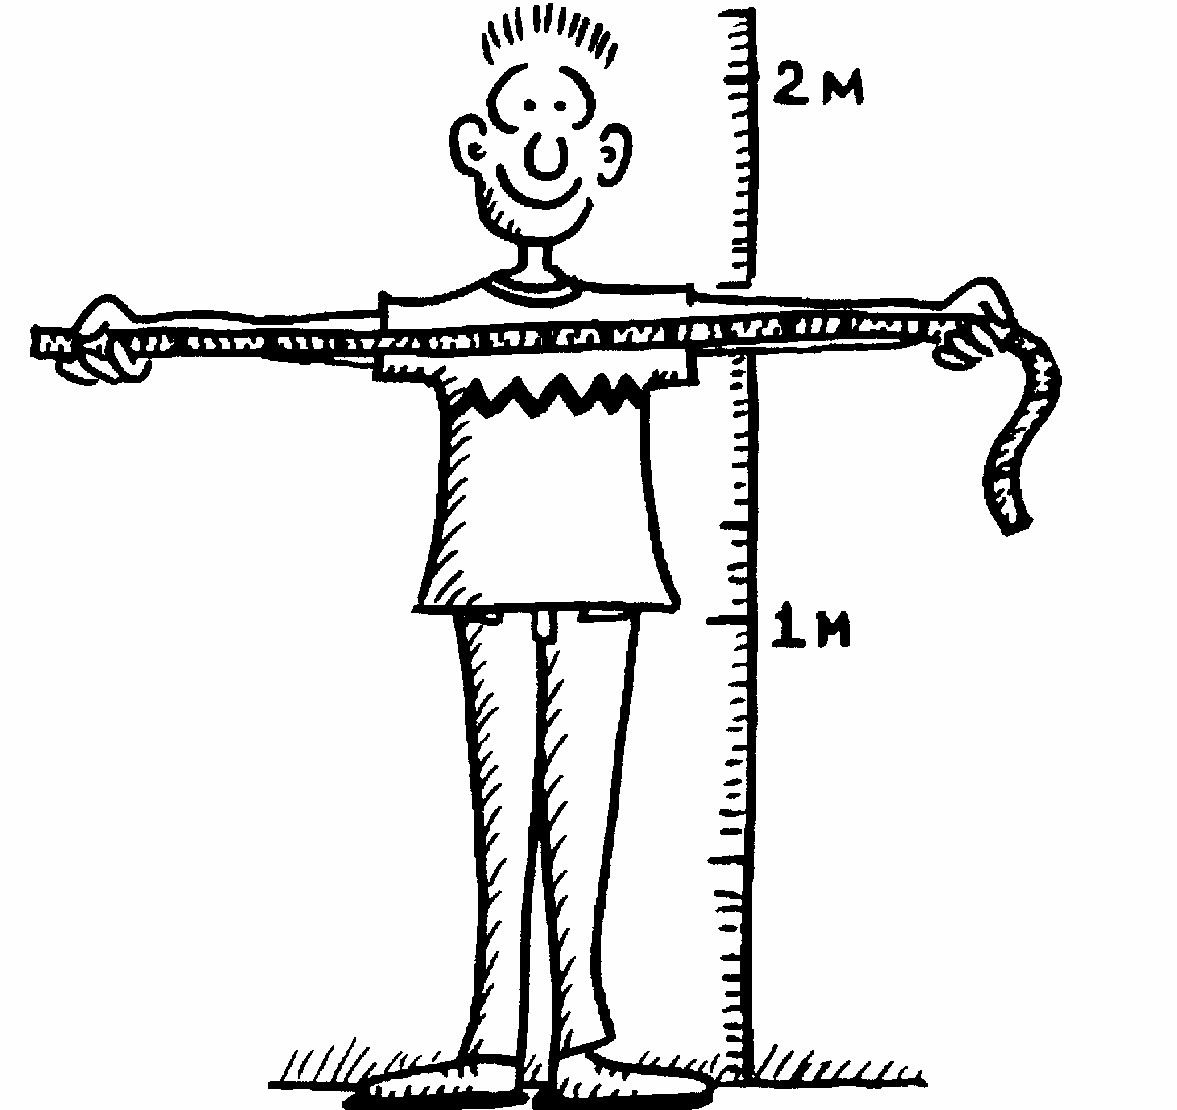
\includegraphics[scale=0.2]{measure-man.jpg}
\end{center}

\vspace{1cm}

{\huge 1. Record the height and armspan of your classmates:}

\vspace{1cm}

\begin{center}
{\large
\begin{tabular}{c|c|c}
\textbf{Name} & \textbf{Height (cm)} & \textbf{Armspan (cm)} \\ \hline
 \hspace{4cm} & & \\ \hline
 & & \\ \hline
 & & \\ \hline
 & & \\ \hline
 & & \\ \hline
 & & \\ \hline
 & & \\ \hline
 & & \\ \hline
 & & \\ \hline
 & & \\ \hline
 & & \\ \hline
 & & \\ \hline
 & & \\ \hline
 & & \\ \hline
 & & \\ \hline
 & & \\ \hline
 & & \\ \hline
 & & \\ \hline
 & & \\ \hline
 & & \\ \hline
 & & \\ \hline
 & & \\ \hline
 & & \\ \hline
 & & \\ \hline
 & & \\ \hline
 & & \\
\end{tabular}
}
\end{center}

\pagebreak

{\huge 2. Construct a scatterplot of Height vs. Armspan by first choosing a scale and labelling the axes, and then  plotting your data.}

\vspace{0.4cm}

\begin{center}
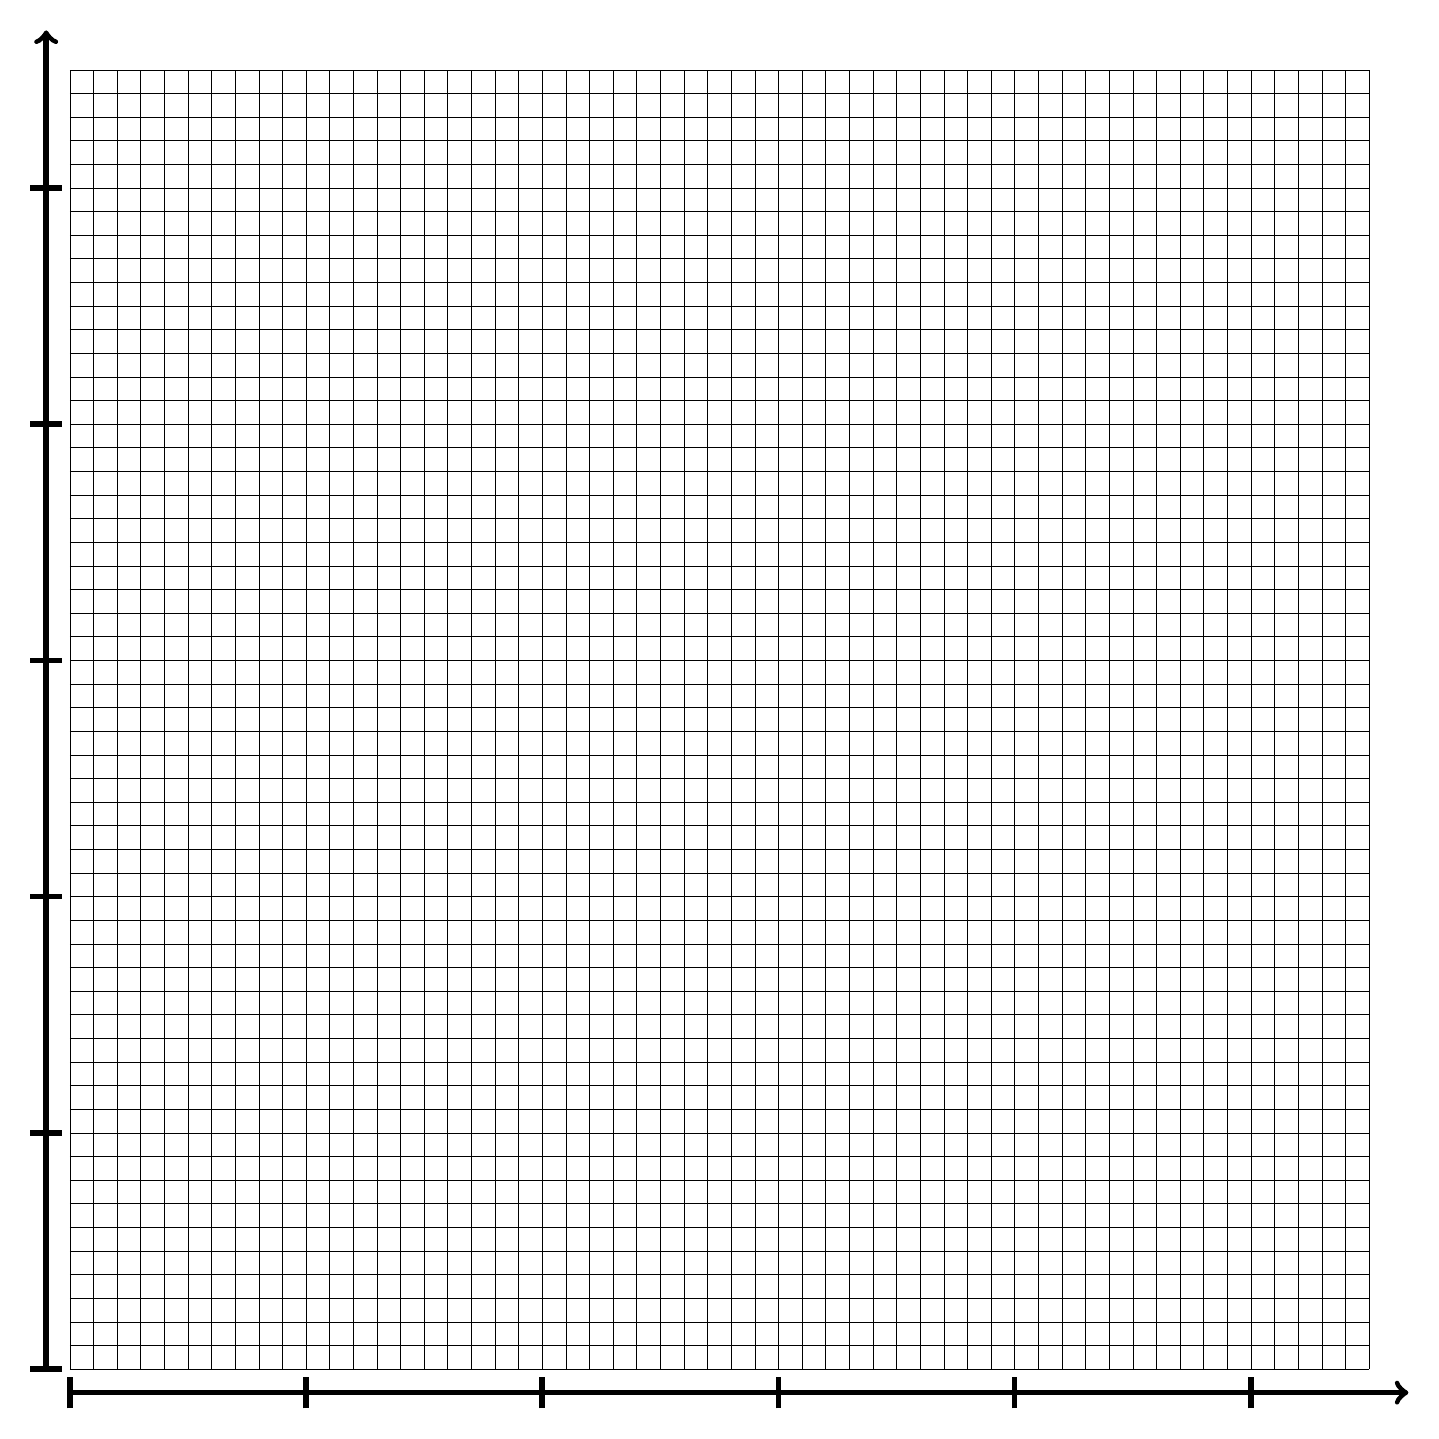
\begin{tikzpicture}
\draw[step=0.3,black,very thin] (0,0) grid (16.5,16.5);
\draw[->, line width = 2pt] (0,-0.3) -- (17, -0.3);
\draw[->, line width = 2pt] (-0.3,0) -- (-0.3, 17);
\draw[line width = 2pt] (0, -0.5) -- (0, -0.1);
\draw[line width = 2pt] (3, -0.5) -- (3, -0.1);
\draw[line width = 2pt] (6, -0.5) -- (6, -0.1);
\draw[line width = 2pt] (9, -0.5) -- (9, -0.1);
\draw[line width = 2pt] (12, -0.5) -- (12, -0.1);
\draw[line width = 2pt] (15, -0.5) -- (15, -0.1);
% \draw (7.5, -0.8) node {\Large Height (cm)};
% \draw (0, -0.8) node  {\Large 140cm};
% \draw (3, -0.8) node  {\Large 150cm};
% \draw (6, -0.8) node  {\Large 160cm};
% \draw (9, -0.8) node  {\Large 170cm};
% \draw (12, -0.8) node {\Large 180cm};
% \draw (15, -0.8) node {\Large 190cm};
\draw[line width = 2pt] (-0.5, 0) -- (-0.1, 0);
\draw[line width = 2pt] (-0.5, 3) -- (-0.1, 3);
\draw[line width = 2pt] (-0.5, 6) -- (-0.1, 6);
\draw[line width = 2pt] (-0.5, 9) -- (-0.1, 9);
\draw[line width = 2pt] (-0.5, 12) -- (-0.1, 12);
\draw[line width = 2pt] (-0.5, 15) -- (-0.1, 15);
% \draw (-1.3, 0.1) node  {\Large 140cm};
% \draw (-1.3, 3.1) node  {\Large 150cm};
% \draw (-1.3, 6.1) node  {\Large 160cm};
% \draw (-1.3, 9.1) node  {\Large 170cm};
% \draw (-1.3, 12.1) node  {\Large 180cm};
% \draw (-1.3, 15.1) node  {\Large 190cm};

\end{tikzpicture}
\end{center}

\vspace{0.4cm}

{\huge 3. Draw the line representing people with the same height as armspan, to seperate people with positive ape index from those with negative ape index.}




\end{document}



